\documentclass[6008notes.tex]{subfiles}
\begin{document}
\graphicspath{ {images/decisions/} }

\section{Decisions and Expectations}

\subsection{Introduction to Decision Making and Expectations}

We now know the basics of working with probabilities. But how do we incorporate probabilities into making decisions?

Let's make this concrete. Suppose we are given the option of playing one of the following lotteries. Which one should we play?

\begin{itemize}
\item Lottery 1: Pay \$1 and have a one in one million chance of winning \$1000.

\item Lottery 2: Pay \$1 and have a one in one million chance of winning \$1000000.

\item Lottery 3: Pay \$1 and have a one in ten chance of winning \$10.
\end{itemize}

Of course, there isn't a right or wrong answer here, but what we would like to do is come up with some quantitative way to make a decision. Especially if we want to make decisions automatically based on huge amount of observations, a principled quantitative approach is crucial!

One way to go about making a decision is to compute as score for each of the possible choices and choose the decision with the highest score. In this case of choosing between the three lotteries, for each of the lotteries, we could compute some kind of ``average'' amount of winnings, accounting for the cost to play.

For example, if we play the first lottery, we definitely lose \$1, and then there is a $\frac{1}{1000000}$ chance that we win \$1,000. So one way we could write out an ``average'' amount of winnings is something like

{\centering$-1+1000\cdot \frac{1}{1000000}=-1+0.001=-0.999.$ \par}
 
For now, multiplying the \$1,000 by $\frac{1}{1000000}$ can be thought of as a heuristic that signifies that we aren't guaranteed to win \$1,000, and how much we multiply by we're just picking to be the probability of winning right now.

Using the above way we have just come up with for computing ``average'' winnings, the second lottery has average winnings

{\centering$-1+\frac{1}{1000000}(1000000)=-1+1=0.$ \par}
 
That's not so bad right? The chance of winning is still really low but the average winnings according to this calculation is 0, so it seems like we stand nothing to lose right?

Well, it depends on how much uncertainty we're willing to tolerate. A one in a million chance seems really low so almost always we would just lose a dollar if we play lottery \#2.

In the third lottery, the average winnings is

{\centering$-1+\frac{1}{10}(10)=0,$ \par}
 
the same as for lottery \#2. Sure, we aren't going to win \$1000000 in this game but the chance of winning is way higher: 1/10 instead of 1/1000000. Somehow that should matter right?

On the basis of the average winnings calculation we have done though, lotteries \#2 and \#3 would be equally good as the give the same highest average winnings of \$0.

We now discuss how to quantitatively and rigorously reason about scenarios like the ones we've just sketched. The main tool we now introduce is what's called the expected value of a random variable. In making decisions that account for randomness, it often makes sense to account for an ``average'' scenario that we should expect. Expectation is about taking an average, accounting for how likely different outcomes are.

In 6.008.1x, after we cover our story here on expected values, we won't be seeing them again until the third part of the course on learning probabilistic models. The idea there is that what probabilistic model makes sense for your data can be thought of as decision making! We are deciding which model to use instead of, in our example here, deciding which lottery to play!

\subsection{The Expected Value of a Random Variable}

Consider, for example, the mean of three values: 3, 5, and 10. It can be computed as follows:

{\centering$\frac{3+5+10}{3}=3\cdot \frac{1}{3}+5\cdot \frac{1}{3}+10\cdot \frac{1}{3}=6.$ \par}
 
Notice, on the right-hand side, that we are adding 3, 5, and 10 each weighted by $\frac{1}{3}$. Concretely, consider a random variable $X$ given by the probability table below:

{\centering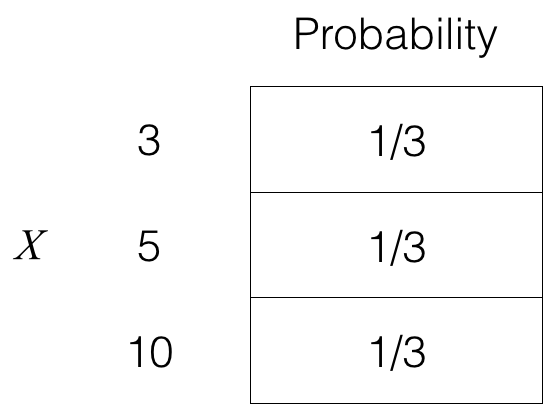
\includegraphics[scale=0.3]{images_sec-expectation-example1} \par}

Then the ``expected value'' of $X$ is given by

{\centering$3\cdot p_{X}(3)+5\cdot p_{X}(5)+10\cdot p_{X}(10)=3\cdot \frac{1}{3}+5\cdot \frac{1}{3}+10\cdot \frac{1}{3}=\frac{18}{3}=6.\dots$ \par}
 
But what if, for instance, we think that 3 is actually much more plausible than 5 or 10? Then what we could do is have the weight on 3 be higher than $\frac{1}{3}$ while decreasing the weights for 5 and 10. Consider if instead we had:

{\centering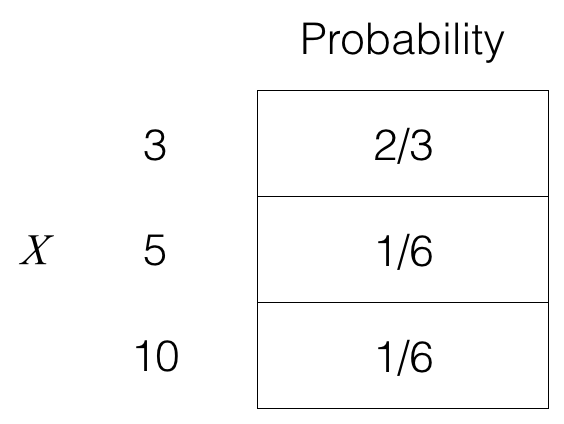
\includegraphics[scale=0.3]{images_sec-expectation-example2} \par}

Then the expected value of $X$ is given by

{\centering$3\cdot p_{X}(3)+5\cdot p_{X}(5)+10\cdot p_{X}(10)=3\cdot \frac{1}{3}+5\cdot \frac{1}{3}+10\cdot \frac{1}{3}=\frac{18}{3}=6.\dots$ \par}
 
Using probability, we now formalize the concept of expected value of a random variable. As you can see, all we are doing is taking the sum of the labels in the probability table, where we weight each label by the probability of the label. \textit{Importantly, the labels are numbers so that it's clear what adding them means!}

Now, for the formal definition:

\paragraph{Definition of expected value:} Consider a real-valued random variable $X$ that takes on values in a set $\mathcal{X}$. Then the expected value of $X$, denoted as $\mathbb {E}[X]$, is

{\centering$\mathbb {E}[X]\triangleq \sum _{x\in \mathcal{X}}x\cdot p_{X}(x).$ \par}
 
Having the random variable be real-valued makes it so that we can add up the labels with weights!

Also, note that whereas $X$ can be represented as a probability table, its expectation $\mathbb {E}[X]$ is just a single number. The expected value is the sum of the values in the set $\mathcal{X}$, weighted by the probabilities of each of the values. The mean is simply the expected value when all of the values in the set $\mathcal{X}$ when there is a uniform probability of each of the values.

Notice that how we came up with the expectation of a random variable $X$ just relied on the probability table for $X$.

In fact, if we took a different probability table, if the labels are numbers, then we can still compute the expectation! Two important examples are below.

\textit{Conditional Expectation}

As a first example, suppose we have two random variables $X$ and $Y$ where we know (or we have already computed) $p_{X\mid Y}(\cdot \mid y)$ for some fixed value $y$, and $X$ is real-valued. Then we can readily compute the expectation for this probability table by multiplying each value $x$ in the alphabet of random variable $X$ by $p_{X\mid Y}(x \mid y)$ and summing these up to get a weighted average. This yields what is called the conditional expectation of $X$ given $Y=y$, denoted as

{\centering$\mathbb {E}[X\mid Y=y]=\sum _{x\in \mathcal{X}}x\cdot p_{X\mid Y}(x\mid y).$ \par}
 
\textit{Expectation of the Function of a Random Variable}

As another example, suppose we have a (possibly not real-valued) random variable $X$ with probability table $p_X$, and we have a function $f$ such that $f(x)$ is real-valued for all $x$ in the alphabet $\mathcal{X}$ of $X$. Then $f(X)$ has a probability table where the labels are all numbers, and so we can compute $\mathbb {E}[f(X)]$.

Let's work out the math here. First, let's determine the probability table for $f(X)$. To make the notation here easier to parse, let random variable $Z=f(X)$. Note that Z has alphabet $\mathcal{Z}=\{ f(x)\; :\; x\in \mathcal{X}\}$. Then the probability table for $f(X)$ can be written as $p_Z$. In terms of the probability table, to compute $p_Z(z)$, we first look at every label in table $p_X$ that gets mapped to $z$, i.e., the set $\{ x\in \mathcal{X}\: :\; f(x)=z\}$. Then we sum up the probabilities of these labels to get the probability that $Z=z$, i.e., $p_{Z}(z)=\sum _{x\in \mathcal{X}\text { such that }f(x)=z}p_{X}(x)$.

We introduce a new piece of notation here called an indicator function $\mathbf{1}\{ \cdot \}$ that takes as input a statement $\mathcal{S}$ and outputs:

\begin{eqnarray*}
\mathbf{1}\{\mathcal{S}\}=\begin{cases}
1 & \text{if }\mathcal{S}\text{ happens},\\
0 & \text{otherwise}.
\end{cases}
\end{eqnarray*}
 
Then the probability that $Z=z$ can be written

\begin{eqnarray*}
p_{Z}(z) &=& \sum _{x\in \mathcal{X}\text { such that }f(x)=z}p_{X}(x) \\
				 &=& \sum _{x\in \mathcal{X}}\mathbf{1}\{ f(x)=z\} p_{X}(x).
\end{eqnarray*}

Next, we compute the expectation of $Z=f(X)$:

\begin{eqnarray*}
\mathbb {E}[Z] &=& \sum _{z\in \mathcal{Z}}zp_{Z}(z) \\
			&=& \sum _{z\in \mathcal{Z}}z\bigg[\sum _{x\in \mathcal{X}}\mathbf{1}\{ f(x)=z\} p_{X}(x)\bigg] \\
			&=& \sum _{x\in \mathcal{X}}\underbrace{\sum _{z\in \mathcal{Z}}z\mathbf{1}\{ f(x)=z\} p_{X}(x)}_{\text {there is only 1 nonzero term here: when }z=f(x)} \\
			&=& \sum _{x\in \mathcal{X}}f(x)p_{X}(x).
\end{eqnarray*}
 
Hence, since $Z=f(X)$, we can write

{\centering$\mathbb {E}[f(X)]=\sum _{x\in \mathcal{X}}f(x)p_{X}(x).$ \par}
 

\subsection{Variance and Standard Deviation}

The variance of a real-valued random variable $X$ is defined as

{\centering$\text {var}(X) \triangleq \mathbb {E}[ (X - \mathbb {E}[X])^2 ].$ \par}
 
Note that as we saw previously, $\mathbb {E}[X]$ is just a single number. To keep the variance of $X$, what you could do is first compute the expectation of $X$.

For example, if $X$ takes on each of the values 3, 5, and 10 with equal probability 1/3, then first we compute $\mathbb {E}[X]$ to get 6, and then we compute $\mathbb {E}[(X - 6)^2]$, where we remember to use the result that for a function $f$, if $f(X)$ is a real-valued random variable, then $\mathbb {E}[f(X)] = \sum _ x f(x) p_ X(x)$. Here, $f$ is given by $f(x) = (x-6)^2$. So

{\centering$\text {var}(X) = (3 - 6)^2 \cdot \frac13 + (5 - 6)^2 \cdot \frac13 + (10 - 6)^2 \cdot \frac13 = \frac{26}{3}.$ \par}


\subsection{Practice Problem: The Law of Total Expectation}

Remember the law of total probability? For a set of events $\mathcal{B}_{1},\dots ,\mathcal{B}_{n}$ that partition the sample space $\Omega$ (so the $\mathcal{B}_{i}$'s don't overlap and together they fully cover the full space of possible outcomes),

{\centering$\mathbb {P}(\mathcal{A})=\sum _{i=1}^{n}\mathbb {P}(\mathcal{A}\cap \mathcal{B}_{i})=\sum _{i=1}^{n}\mathbb {P}(\mathcal{A}\mid \mathcal{B}_{i})\mathbb {P}(\mathcal{B}_{i}),$ \par}
 
where the second equality uses the product rule.

A similar statement is true for the expected value of a random variable, called the law of total expectation: for a random variable $X$ (with alphabet $\mathcal{X}$) and a partition $\mathcal{B}_{1},\dots ,\mathcal{B}_{n}$ of the sample space,

{\centering$\mathbb {E}[X]=\sum _{i=1}^{n}\mathbb {E}[X\mid \mathcal{B}_{i}]\mathbb {P}(\mathcal{B}_{i}),$ \par}
 
where

{\centering$\mathbb {E}[X\mid \mathcal{B}_{i}] = \sum _{x\in \mathcal{X}}xp_{X\mid \mathcal{B}_{i}}(x) = \sum _{x\in \mathcal{X}}x\frac{\mathbb {P}(X=x,\mathcal{B}_{i})}{\mathbb {P}(\mathcal{B}_{i})}.$ \par}
 
We will be using this result in the section ``Towards Infinity in Modeling Uncertainty''.

Show that the law of total expectation is true.

\paragraph{Solution:} There are different ways to prove the law of total expectation. We take a fairly direct approach here, first writing everything in terms of outcomes in the sample space.

The main technical hurdle is that the events $\mathcal{B}_{1},\dots ,\mathcal{B}_{n}$ are specified directly in the sample space, whereas working with values that $X$ takes on requires mapping from the sample space to the alphabet of $X$.

We will derive the law of total expectation starting from the right-hand side of the equation above, \\ i.e., $\sum _{i=1}^{n}\mathbb {E}[X\mid \mathcal{B}_{i}]\mathbb {P}(\mathcal{B}_{i})$.

We first write $\mathbb {E}[X\mid \mathcal{B}_{i}]$ in terms of a summation over outcomes in $\Omega$:

{\centering{\renewcommand{\arraystretch}{1.5}
\begin{tabular}{l l l}
$\mathbb {E}[X\mid \mathcal{B}_{i}]$ & $=$ & $\sum _{x\in \mathcal{X}}x\frac{\mathbb {P}(X=x,\mathcal{B}_{i})}{\mathbb {P}(\mathcal{B}_{i})}$ \\
  & $=$ & $\sum _{x\in \mathcal{X}}x\frac{\mathbb {P}(\{ \omega \in \Omega \; :\; X(\omega )=x\} \cap \mathcal{B}_{i})}{\mathbb {P}(\mathcal{B}_{i})}$ \\
  & $=$ & $\sum _{x\in \mathcal{X}}x\frac{\mathbb {P}(\{ \omega \in \Omega \; :\; X(\omega )=x\text { and }\omega \in \mathcal{B}_{i}\} )}{\mathbb {P}(\mathcal{B}_{i})}$ \\
  & $=$ & $\sum _{x\in \mathcal{X}}x\frac{\mathbb {P}(\{ \omega \in \mathcal{B}_{i}\; :\; X(\omega )=x\} )}{\mathbb {P}(\mathcal{B}_{i})}$ \\
  & $=$ & $\sum _{x\in \mathcal{X}}x\cdot \frac{\sum _{\omega \in \mathcal{B}_{i}\text { such that }X(\omega )=x}\mathbb {P}(\{ \omega \} )}{\mathbb {P}(\mathcal{B}_{i})}$ \\
  & $=$ & $\frac{1}{\mathbb {P}(\mathcal{B}_{i})}\sum _{x\in \mathcal{X}}x\sum _{\omega \in \mathcal{B}_{i}\text { such that }X(\omega )=x}\mathbb {P}(\{ \omega \} )$ \\
  & $=$ & $\frac{1}{\mathbb {P}(\mathcal{B}_{i})}\sum _{\omega \in \mathcal{B}_{i}}X(\omega )\mathbb {P}(\{ \omega \} ).$ 
\end{tabular}} \par}
		
Thus,

{\centering{\renewcommand{\arraystretch}{1.5}
\begin{tabular}{l l l}
$\sum _{i=1}^{n}\mathbb {E}[X\mid \mathcal{B}_{i}]\mathbb {P}(\mathcal{B}_{i})$ & $=$ & $\sum _{i=1}^{n}\bigg(\frac{1}{\mathbb {P}(\mathcal{B}_{i})}\sum _{\omega \in \mathcal{B}_{i}}X(\omega )\mathbb {P}(\{ \omega \} )\bigg)\mathbb {P}(\mathcal{B}_{i})$ \\
  & $=$ & $\sum _{i=1}^{n}\sum _{\omega \in \mathcal{B}_{i}}X(\omega )\mathbb {P}(\{ \omega \} )$ \\
  & $=$ & $\sum _{\omega \in \Omega }X(\omega )\mathbb {P}(\{ w\} )$ \\
  & $=$ & $\sum _{x\in \mathcal{X}}x\mathbb {P}(\{ \omega \in \Omega \text { such that }X(\omega )=x\} )$ \\
  & $=$ & $\sum _{x\in \mathcal{X}}xp_{X}(x)$ \\
  & $=$ & $\mathbb {E}[X].$ \\
\end{tabular}} \par}



\end{document}
